\documentclass{beamer}
\usepackage[utf8]{inputenc}
\usepackage[slovene]{babel}
\usepackage{amsmath}
\usepackage{mathtools}
\usepackage{multicol}
\usetheme{Madrid}
\setbeamertemplate{navigation symbols}{}

\title[Razširjanje zaupanja]{Razširjanje zaupanja za lokalizacijo senzorskih omrežji}
\author{Jaka Velkaverh}
\date{18.12.2023}

\theoremstyle{definition}
\newtheorem{definicija}{Definicija}

\begin{document}

	\frame{\titlepage}

	\begin{frame}
		\frametitle{Opis problema}
		\begin{block}{Lokalizacija senzorskega omrežja}
			Omrežje si predstavljamo kot utežen graf, kjer so naprave vozlišča.
			Dve vozlišči sta povezani, če sta pripadajoči napravi dovolj blizu,
			da lahko izmerita razdaljo. Utež povezav je izmerjena razdalja,
			kjer pri merjenju pride do napak.

			Vemo lokacije od nekaterih naprav, tem rečemo sidra. Izračunati
			želimo približke za lokacije ostalih, tem rečemo agenti.
		\end{block}
		Predpostavimo, da je omrežje naprav povezano.
	\end{frame}

	\begin{frame}
		\frametitle{Verjetnostni pogled}
		Oznake
		\begin{itemize}
			\item Vozlišča označujemo z črkami $u, v, s$.
			\item Napaka pri merjenju $\nu_{u, v} \sim N\left(0, \sigma^2\right)$.
			\item $\underline{X}_u \in K\left(0,R\right) \subseteq \mathbb{R}^n$ naključni vektor lokacije naprave.
			\item $\underline{X}_A$ naključni vektor lokacije množice naprav $A$.
		\end{itemize}
	\end{frame}

	\begin{frame}
		\frametitle{Markovska polja}
		\begin{block}{Pogojna neodvisnost}
			Nakjučna vektorja $\underline{X}, \underline{Y}$ sta pogojno
			neodvisna ob $\underline{Z}$, če velja:
			$$f_{\underline{X}, \underline{Y}}\left(\underline{x}, \underline{y}\ |\ \underline{Z} = \underline{z}\right) =
			  f_{\underline{X}}\left(\underline{x}\ |\ \underline{Z} = \underline{z}\right) \
			  f_{\underline{Y}}\left(\underline{y}\ |\ \underline{Z} = \underline{z}\right)
			$$
		\end{block}
		\pause
		\begin{definicija}
			Graf $G = \left(V, E\right)$, in naključni slučajni vektorji
			$\underline{X}_v$, indeksirani z $v \in V$ tvorijo Markovsko polje,
			če velja Markova lastnost po parih:

			Za vsaka nesosedna $u, v \in V$ sta $\underline{X}_u$, $\underline{X}_v$
			pogojno neodvisna ob vseh ostalih
			$\underline{X}_{V\backslash\left\{u, v\right\}}$
		\end{definicija}
	\end{frame}

	\note{
		Intuitivno ima naš problem strukturo Markovskega polja.
		Vozlišča identificiramo z naključnimi vektorji naprav, povežemo pa tista vozlišča,
		ki so lahko izmerila medsebojno razdaljo. Če potem pogledamo dve nesosedni vozlišči,
		pripadajoča vektorja gotovo ne bosta neodvisna, saj sta povezana z neko poti.
		Vsak soseden par na tej poti je odvisen, torej bosta oba konca poti posredno
		preko vseh vmesnih vozlišč odvisna.

		Če pa fiksiramo vrednosti vseh vozlišč, pa bosta neodvisna. V tem primeru vozlišči
		ne vplivata na sosede, saj imajo te fiksno vrednost, ker pa sama nista soseda,
		bosta torej neodvisna.

		Seveda je to samo intuitivnem nivoju.
	}

	\begin{frame}
		\begin{block}{Hammersley–Cliffordov izrek}
			Naj bo $G = \left(V, E\right)$ in $\underline{X}_v$ kot prej in dodatno
			$f_{\underline{X}_V}\left(\underline{x}_V\right) > 0\quad \forall \underline{x}_V$.
			Tedaj $G$ in $\underline{X}_V$ tvorita Markovsko polje natanko tedaj,
			ko se skupna gostota faktorizira po klikah grafa $G$:
			$$f_{\underline{X}_V}\left(\underline{x}_V\right) \propto
				\prod_{C\;\text{klika}\;G}\psi_C\left(\underline{x}_C\right)$$
		\end{block}
		\pause
		Torej če definiramo skupno gostoto kot produkt potencialov, bodo
		pripadajoče slučajne spremenljivke tvorile Markovsko polje.
	\end{frame}

	\note{
		Izrek nam ob šibkem pogoju, da je gostota povsod pozitivna natanko opiše vse skupne
		porazdelitve Markovskih polj.

		Členom $\psi$ pravimo potenciali po vzoru iz fizike.
	}

	\begin{frame}
		Za $\left\{u,v\right\} \in E$ in $d_{u,v}$ izmerjena razdalja definiramo
		$$
		\psi_{u,v}\left(\underline{x}_u,\underline{x}_v\right) =
		f_{\nu_{u, v}}\left(\left|\underline{x}_u-\underline{x}_v\right| - d_{u,v}\right) =
		\frac{1}{\sigma\sqrt{2\pi}} \exp\left[-\frac{\left(\left|\underline{x}_u-\underline{x}_v\right| - d_{u,v}\right)^2}{2 \sigma^2}\right]
		$$
		Za klike $C$, ki niso velikosti $2$
		$$
		\psi_C\left(\underline{x}_C\right)=1
		$$
		Po izreku bo produkt takih potencialov skupna porazdelitev nekega slučajnega vektorja,
		ki ima strukturo Markovskega polja.
	\end{frame}

	\note{
		Problem se v resnici rešuje v obratni smeri. Najprej definiramo smiseln izraz,
		ki ga želimo maksimizirati, nato pa opazimo, da je v resnici skupna gostota
		neke porazdelitve, ki ima strukturo, ki jo je smiselno pričakovati od začetnega
		problema.

		V resnici se maksimiziranje produkta potencialov prevede na minimiziranje kvadrata
		razlike razdalje, izračunane iz predvidenih lokacij naprav in izmerjene razdalje.
		Torej smo začeli s problemom najmanjših kvadratov.
	}

	\begin{frame}
		\begin{figure}[t]
			\includegraphics[width=7cm]{"pairwise_potential.png"}
			\caption{Primer potenciala parov, če eno od pozicij fiksiramo. Tu je izmerjena razdalja $10$, $\sigma$ pa $0{,}3$.}
			\centering
		\end{figure}
	\end{frame}

	\begin{frame}
		Naj bodo $V_a$ agenti, $V_s$ pa sidra.
		Z $\underline{y}_{V_s}$ označimo (fiksne) znane pozicije sider.
		Posteriorna gostota bo torej
		$$
		f_{V_a | V_s}\left(\underline{x}_{V_a} | V_s = \underline{y}_{V_s}\right) \propto
		\prod_{\substack{\left\{u,v\right\} \in E \\ u,v \text{ agenta}}}\psi_{u,v}\left(\underline{x}_u,\underline{x}_v\right)
		\prod_{\substack{\left\{u,v\right\} \in E \\ u\text{ agent}, v \text{ sidro}}}\psi_{u,v}\left(\underline{x}_u,\underline{y}_v\right)
		$$
		\pause
		Za $u \in V_a$ želimo izračunati robno gostoto
		$$
		f_{X_u | V_s}\left(\underline{x}_u | V_s = \underline{y}_{V_s}\right) =
		\int_{V_a\backslash X_u} f_{V_a | V_s}\left(\underline{x}_{V_a\backslash X_u} | V_s = \underline{y}_{V_s}\right)
		d\underline{x}_{V_a\backslash X_u}
		$$
	\end{frame}

	\note{
		Skupna gostota je funkcija zelo veliko spremenljivk in je zato precej
		okorna. Ljubše nam bi bilo, če bi jo lahko poenostavili na funkcijo vektorja
		samo ene naprave. Ker problem rešujemo v okviru verjetnosti bomo to dosegli tako,
		da izračunamo robno verjetnost (marginalization).
	}

	\begin{frame}
		\frametitle{Razširjanje zaupanja na drevesih}
		Poglejmo si primer, ko je graf drevo.
		\setlength{\columnsep}{-3.5cm}
		\begin{multicols}{2}
			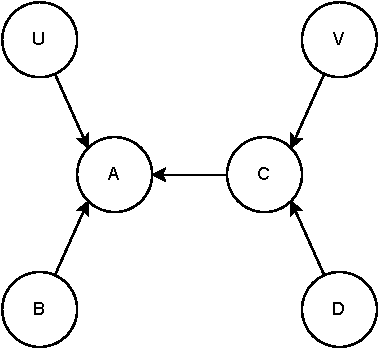
\includegraphics[width=4cm]{message_passing.pdf}
			\columnbreak{}

			$$
			\int_{V_a\backslash X_u} f_{V_a | V_s}\left(\underline{x}_{V_a\backslash X_A} | V_s = \underline{y}_{V_s}\right)
			d\underline{x}_{V_a\backslash X_A} \propto
			$$
			$$
			\int_{\underline{X}_B,\underline{X}_D,\underline{X}_C} \psi_{U,A} \psi_{B,A} \psi_{C,A} \psi_{V,C} \psi_{D,C}d\underline{x}_Bd\underline{x}_Dd\underline{x}_C =
			$$
			\pause
			$$
			\psi_{U,A} \int \psi_{B,A}d\underline{x}_B \int \psi_{C,A} \psi_{V,C}
			\int \psi_{D,C}d\underline{x}_Dd\underline{x}_C=
			$$
		\end{multicols}
	\end{frame}

	\note{
		Tu na konkretnem primeru drevesa vidimo, da se integral skupne gostote poenostavi.
	}

	\begin{frame}
		\begin{align*}
			\text{Za } u,v \in V_a\text{: } &
			\mu_{u \to v}\left(\underline{x}_v\right) \coloneqq
			\int \psi_{u,v}\left(\underline{x}_u,\underline{x}_v\right)
			\prod_{t\in N\left(u\right)\backslash v}
			\mu_{t \to u}\left(\underline{x}_u\right)d\underline{x}_u
			\\
			\text{Za }u \in V_s\text{ in }v \in V_a\text{: } &
			\mu_{u \to v}\left(\underline{x}_v\right) \coloneqq
			\psi_{u,v}\left(\underline{y}_u,\underline{x}_v\right)
		\end{align*}
		\pause
		$$
		\Rightarrow
		\psi_{U,A} \int \psi_{B,A}d\underline{x}_B \int \psi_{C,A} \psi_{V,C}
		\int \psi_{D,C}d\underline{x}_Dd\underline{x}_C=
		$$
		\pause
		$$
		\mu_{U \to A}\left(\underline{x}_A\right)\mu_{B \to A}\left(\underline{x}_A\right)
		\int \psi_{C,A}
		\mu_{V \to C}\left(\underline{x}_C\right)
		\mu_{D \to C}\left(\underline{x}_C\right)d\underline{x}_C=
		$$
		\pause
		$$
		\mu_{U \to A}\left(\underline{x}_A\right)\mu_{B \to A}\left(\underline{x}_A\right)
		\mu_{C \to A}\left(\underline{x}_A\right) =
		$$
		$$
		\prod_{u \in N\left(A\right)}\mu_{u \to A}\left(\underline{x}_A\right)
		$$
	\end{frame}

	\note{
		Če tu definiramo sporočila $\mu_{u \to v}$ med vozlišči, se računanje
		robne gostote poenostavi na računanje sporočil. Ker usmerjeni grafi brez
		ciklov premorejo topološko ureditev, je definicija sporočil dobra.
		V vsakem drevesu obstaja zaporedje računanja sporočil, z katerim
		imamo v vsakem koraku že izračunana vsa sporočila, ki so potrebna,
		da izračunamo naslednje sporočilo.

		Opazimo, da so sporočila v celoti lokalna. Za njihov izračun so
		potrebna vsa ostala sporočila, ki so prišla do pošiljatelja in potencial
		med pošiljateljem in prejemnikov, za katera pa moramo vedeti le izmerjeno
		razdaljo med vozlišči. Dejansko lahko sporočila računamo distribuirano,
		kar nam omogoči, da naravno uporabimo računsko moč vseh naprav v
		velikem omrežju.

		Opisan postopek ni izvedljiv za grafe s cikli, saj nam cikel da
		krožne zahteve za izračun sporočil.
	}

	\begin{frame}
		\frametitle{Za grafe s cikli}
		Naj bosta $u,v \in V_a$, $i \in \mathbb{N}$ pa število iteracije.
		$$
		M_u^{\left(i\right)}\left(\underline{x}_u\right) \coloneqq
		\prod_{t \in N\left(u\right)}\mu_{t \to u}\left(\underline{x}_u\right)
		$$
		$$
		\mu_{v \to u}^{\left(i\right)}\left(\underline{x}_u\right) \coloneqq
		\int \psi_{v,u}\left(\underline{x}_v,\underline{x}_u\right)
		\frac{
			M_v^{\left(i-1\right)}\left(\underline{x}_v\right)}{
			\mu_{u \to v}^{\left(i-1\right)}\left(\underline{x}_v\right)
		}d\underline{x}_v
		$$
		Za drevesa to konvergira k pravim vrednostim.
	\end{frame}

	\note{
		Tu je potrebno dodati, da za $i=0$ vrednosti nastavimo na konstantno $1$.
		Funkcijam $M$ pravimo zaupanje. Želimo, da bi konvergirali k robnim gostotam
		porazdelitve.

		Dejanskega zagotovila o konvergenci k pravim vrednostim nimamo.
		V splošnem je problem točne marginalizacije NP - težek. V praksi se pa
		izkaže (kar je tudi delno teoretično utemeljeno), da po nekaj iteracijah
		zaupanje pride do razmeroma natančnih približkov za robne gostote.
	}

\end{document}

